\documentclass[conference]{IEEEtran}
\usepackage[utf8]{inputenc}    % for UTF-8 encoding
\usepackage{amsmath, amssymb}  % for math symbols and equations
\usepackage{graphicx}          % for including graphics
\usepackage{cite}              % for managing citations
\usepackage{url}               % for handling URLs
\usepackage{fancyhdr}  % Package for customizing headers and footers
\usepackage{lipsum}    % Package for generating random text
\usepackage{smartdiagram} % Use Circular Diagram for illustration purposes
\usepackage{xcolor} % For colored Text
\usepackage{tikz} % For producing vector graphics images

% Template inspired by IEEEtran
% Written by Puneet Sharma (UiT The Arctic University of Norway)
% This template should be used for Machine Vision reports

% Set up the header
\fancypagestyle{plain}{
    \fancyhf{} % Clear all header and footer fields
    \fancyhead[C]{\color{red}----- Machine Vision Report - Not Peer Reviewed ------}
    \fancyfoot[C]{\thepage} % Center footer
    \renewcommand{\headrulewidth}{1pt} % No header rule
    \renewcommand{\footrulewidth}{1pt} % No footer rule
}


\pagestyle{plain}


\title{Machine Vision Project Report Title}

\author{
    \IEEEauthorblockN{Candidate no 11, 23, and 71}    
}

\begin{document}

\maketitle

\begin{abstract}
    This is the abstract of the report. Our objective in this report is to ... In this report, we tried N experiments with different parameters to evaluate the XYZ model for the task of classifying DEF. Our results indicate for experiment 1, ABC performs better than DEF by 5 percent, we explain these results in more detail in the discussion section. 
    \\
    \color{red}
    \textbf{This document is compiled based on the commonly asked questions from the students, hence, it is important to read through the entirety of this document carefully.}
    \color{black}
   
   
\end{abstract}

\begin{IEEEkeywords}
    Deep Learning, supervised learning, SGD
\end{IEEEkeywords}



\section{Introduction}
This is the introduction section. In the introduction, we briefly discuss the objective of the report and the overall importance of working towards the objective.
Also, here is how we cite a webpage~\cite{webpage_example}.
Here is how we cite a classic book that was published in 2006~\cite{Gonzalez2006}.
And here is how we cite a book that is under publication or under review~\cite{scardapane2024book}. We would notice in the References section of this report that for most classic and standard books e.g.~\cite{Gonzalez2006}  there is a publisher name, publication date, edition, and year, and if a book e.g,~\cite{scardapane2024book} is under review or publication then it would be lacking these details.

\section{Bullet Points Example}

Some important points to consider:

\begin{itemize}
    \item The maximum length of the report including references is 10 pages.
    \item The report should be delivered as a PDF.
    \item I have written the majority of the text of this example report in \textit{main.tex} file, other options are also OK. 
    \item Use the candidate number provided by WiseFlow.
    \item If you would like to share your GitHub code in the report, it is possible to anonymize it using \url{https://anonymous.4open.science/}
    \item For citing (referencing) research papers, technical reports, and webpages properly we can use a .bib file that can be edited. For example, I have used references.bib file in this project, See the examples in this project.
    \item It is important that the references be valid resources such as research articles, books, academic websites, and \textbf{not random blogs}.
    \item All figures used in the example report are placed under a folder called figures in the project.
    \item Just because I have itemized or used bullet points in the text does not mean that all text should be written in this way. Hence, use bullet points (or item) when necessary.
    \item It is fine to cite (refer) to the same article or book multiple times in a report.
\end{itemize}

\subsection{Specific Concept or Topic}

We use subsections where it is necessary to structure the text.
\begin{figure}[h]
    \centering
    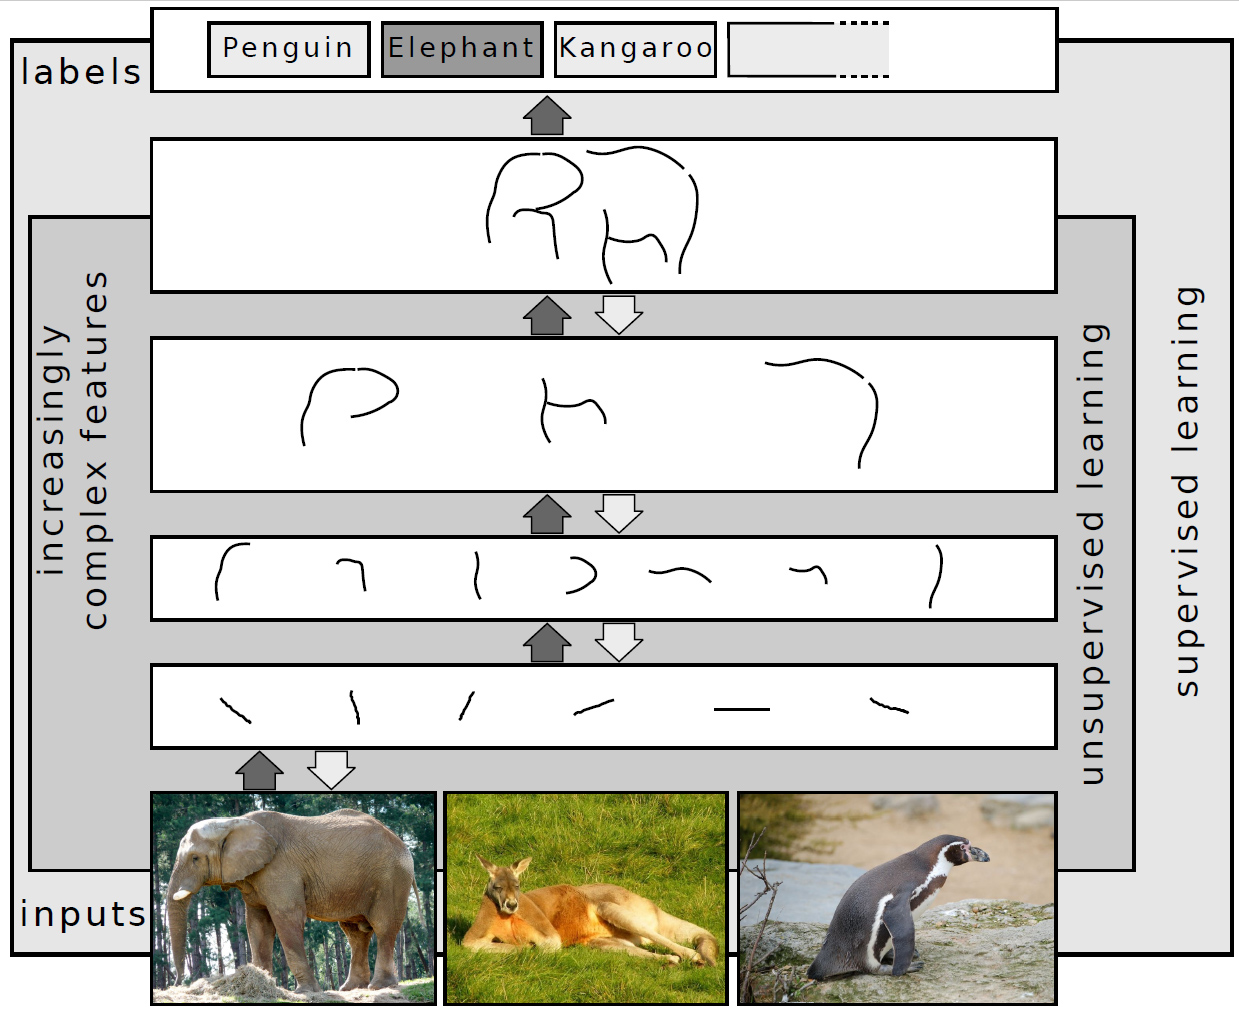
\includegraphics[width=0.45\textwidth]{figures/Deep_Learning.jpg}
    \caption{An example JPG image that should be cited and discussed in the text.  Original source~\cite{schulz2012}}
    \label{fig:example_image}
\end{figure}

It is important to refer to the Figure in the text. For example, Figure~\ref{fig:example_image} shows an example of the difference between supervised and unsupervised learning aspects of a deep learning model.

\section{Theory}
In this section, we explain the theory behind the deep learning model and the hyperparameters used. In the theory section, we can also write about the methods or metrics used for evaluating the performance of the deep learning models.

\subsection{Data}
\begin{itemize}
    \item We can discuss briefly the data used for our experiments here. Show a few images if necessary.
\end{itemize}

\section{Methodology}
This section explains the methodology.
The experiment design i.e., the choice of models used for our experiments, the number of experiments performed with one or multiple deep learning models, and their details such as hyperparameters used. 



\section{Results}
This section presents the results.

\begin{itemize}
    \item It is natural to show how the different models perform better or worse compared to one another or a standard method.
    \item For example, relevant figures and graphs related to the training, validation, and evaluation. Figures should follow with text describing how loss or accuracy is changing over each epoch or iteration.
    \item We can plot the loss and accuracy here and write a bit about the trends that we observe in the data.
    \item In addition, we can also show a few example images for the case when the model or models performed accurately and a few example images when the model or models performed poorly.


\end{itemize}

\begin{figure}[h]
    \centering
    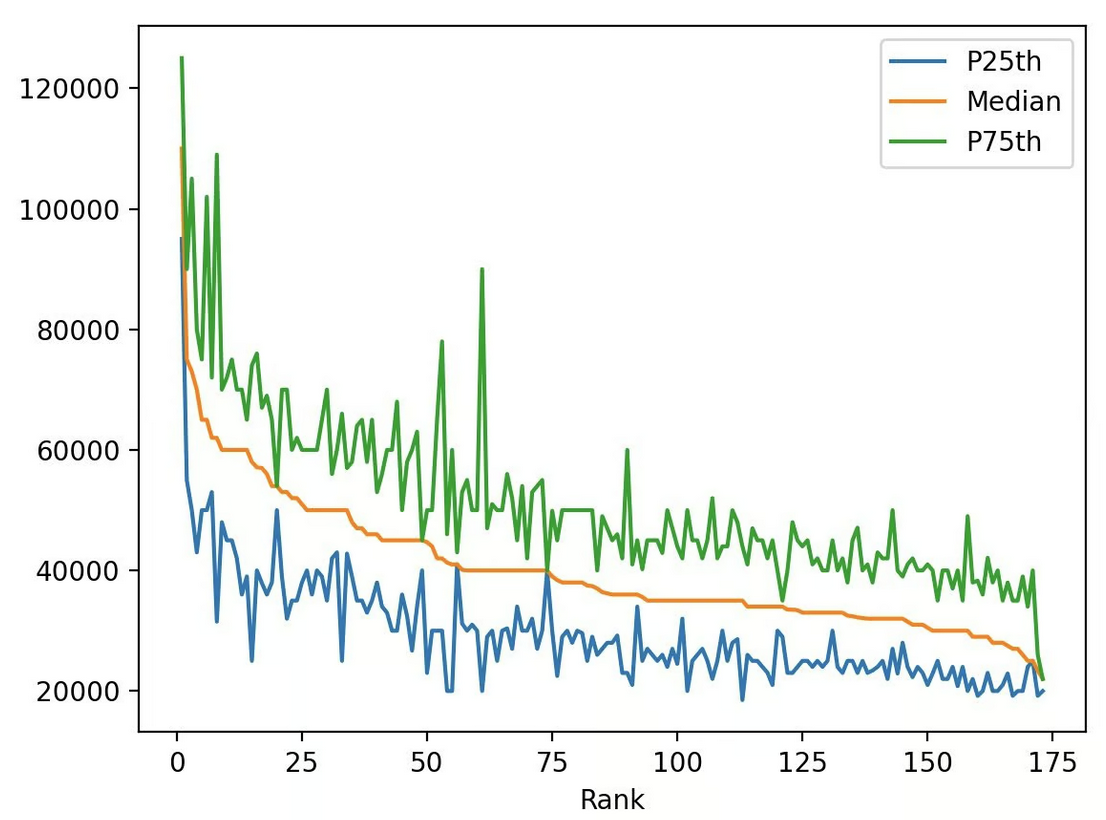
\includegraphics[width=0.45\textwidth]{figures/example_data_plot.png}
    \caption{An example PNG image that shows the results. It is important to have labels on both axes or legends that denote the different data in the plot. Original source~\cite{data_plot_example}}
    \label{fig:example_data}
\end{figure}

We refer to the data in the text here~\ref{fig:example_data} i.e., by using the label text written the figure, the different figures must have different labels. Otherwise, it would generate errors in the latex compiler.

\section{Discussion}


\begin{itemize}
    \item In addition to the positive results, feel free to discuss negative results and possible reasons behind the negative results.
    \item Justification of important choices can be made here, and often this can be linked to results. 
    \item Here we discuss the details of the results for example, why one model with certain hyperparameters is better than another model with same or different hyperparameters.
    \item If any interesting discoveries have been made during the experiments, these should be mentioned here even if they are not important for the project.
    \item Conclusion should not be a copy of the discussion.
\end{itemize}
\section{Conclusion}
This section concludes the report. 
In conclusion, we conclude based on our experiments and results.


\color{black}
\bibliographystyle{IEEEtran}
\bibliography{references}


\end{document}